% SC2001 — Chapter 7: Graph Traversal, Shortest Paths, and String Matching
% No \documentclass — this file is \input/\include'd by main.tex.
\chapter{Graph Traversal, Shortest Paths, and String Matching}
\label{ch:graph-string}

\begin{quote}
\emph{``Graphs and strings are not different worlds.''} BFS discovers distance
as surely as KMP discovers pattern: both exploit structure to avoid redundant work.
\end{quote}

\noindent\textbf{Prerequisites:} Chapter~1 (invariants), Chapter~2 (asymptotics, heaps), and basic graph notation $G=(V,E)$ directed or undirected, $|V|=n$, $|E|=m$.

\section*{Learning Outcomes}
After this chapter you will be able to:
\begin{enumerate}[label=(L\arabic*)]
    \item trace BFS/DFS, explain queue/stack roles and analyse $O(n+m)$ time;
    \item implement Dijkstra with a binary heap and prove correctness via its set invariant;
    \item run Bellman--Ford, detect negative cycles, and derive Floyd--Warshall as DP over $k$;
    \item compute the KMP prefix function $\pi$, simulate its automaton, and analyse Rabin--Karp rolling hash.
    \item run Ford--Fulkerson on small networks, explain residual graphs, and state the max-flow min-cut theorem.
\end{enumerate}

% ============================================================
\section{Graph Traversal: BFS and DFS}
\label{sec:bfs-dfs}

Let $G=(V,E)$ be unweighted for traversal; weights return in \S\ref{sec:shortest}.
\paragraph{How to store a graph?} Think of friends: a \emph{matrix} is a full $n\times n$ attendance sheet (1 if $i$ knows $j$) --- $\Theta(n^2)$ even for a sparse class; a \emph{list} stores only who each person actually knows. We use adjacency lists: for each $v$ keep its neighbour list; scanning all edges costs $\Theta(n+m)$, not $\Theta(n^2)$.
\begin{figure}[h]\centering\begin{tikzpicture}[scale=0.68,every node/.style={font=\scriptsize}]
\node[circle,draw,thick,fill=blue!14,minimum size=7mm] (1) at (0,1.2) {1}; \node[circle,draw,thick,fill=green!14,minimum size=7mm] (2) at (1.8,1.2) {2}; \node[circle,draw,thick,fill=orange!14,minimum size=7mm] (3) at (0,0) {3}; \node[circle,draw,thick,fill=violet!14,minimum size=7mm] (4) at (1.8,0) {4};
\draw[thick,->] (1)--(2); \draw[thick,->] (1)--(3); \draw[thick,->] (2)--(4);
\node[draw,rounded corners,fill=gray!6,font=\tiny,align=left] at (5.2,1.0) {list: $1\!\to\![2,3]$\\ $2\!\to\![4]$\\ $3\!\to\![]$\\ $4\!\to\![]$};
\node[draw,fill=gray!6,font=\tiny] at (5.2,0.0) {$\begin{smallmatrix}0&1&1&0\\0&0&0&1\\0&0&0&0\\0&0&0&0\end{smallmatrix}$ matrix};
\node[font=\tiny,gray] at (2.6,-0.85) {Left: sparse graph. Right: list stores 3 entries vs 16 in matrix.};
\end{tikzpicture}\caption{Adjacency lists vs matrix --- lists pay for edges present, matrices pay for all pairs.}\label{fig:adj-storage}\end{figure}

\subsection{BFS: Queue and Layering}
\paragraph{Queue = line, Stack = pile.} A \emph{queue} is a supermarket line: first in, first out (FIFO) --- you leave in the order you arrived. A \emph{stack} is a pile of plates: last in, first out (LIFO) --- you take the top plate. BFS uses a line (fair: all distance-1 vertices before distance-2); DFS uses a pile (commit deep, backtrack). Same graph, swapped container, different order.
\textsc{BFS}$(G,s)$ explores in waves of increasing distance from source $s$.
It uses a FIFO \emph{queue} $Q$: $s$ is enqueued, then repeatedly dequeued, and each undiscovered neighbour is enqueued.

\begin{quote}\ttfamily\scriptsize
\textsc{BFS}$(G,s)$: dist$[s]\gets0$; $Q\gets[s]$; visited$\gets\{s\}$\\
\textbf{while} $Q\neq\emptyset$: $u\gets\textsc{Dequeue}(Q)$\\
\textbf{for} each $(u,v)\in E$: \textbf{if} $v\notin$ visited \textbf{then} dist$[v]\gets$dist$[u]+1$; parent$[v]\gets u$; \textsc{Enqueue}$(Q,v)$
\end{quote}

\begin{figure}[h]\centering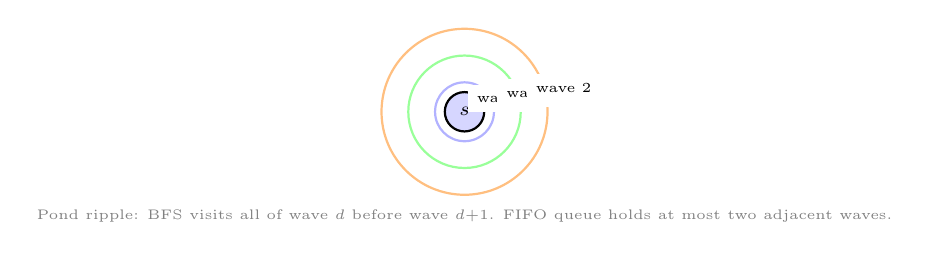
\begin{tikzpicture}[scale=0.68,every node/.style={font=\scriptsize}]
\draw[blue!30,thick] (0,0) circle (0.55); \draw[green!40,thick] (0,0) circle (1.05); \draw[orange!50,thick] (0,0) circle (1.55);
\node[circle,draw,thick,fill=blue!16,minimum size=5mm] at (0,0) {$s$}; \node[font=\tiny,fill=white] at (0.75,0.25) {wave 0};
\node[font=\tiny,fill=white] at (1.30,0.35) {wave 1}; \node[font=\tiny,fill=white] at (1.85,0.45) {wave 2};
\node[font=\tiny,gray,align=center] at (0,-1.95) {Pond ripple: BFS visits all of wave~$d$ before wave~$d{+}1$. FIFO queue holds at most two adjacent waves.};
\end{tikzpicture}\caption{Wave-front view of BFS --- distance layers expand like ripples; the queue is the line of people in ripple order.}\label{fig:bfs-wave}\end{figure}
The \emph{layering} property: $Q$ always contains vertices of at most two consecutive distances $d,d+1$ from $s$, all $d$ before $d+1$. Hence dist$[v]$ is the shortest-path distance $\delta(s,v)$ in an unweighted graph (proved by induction on $d$). Parent pointers form a \emph{BFS tree} rooted at $s$; every non-tree edge connects vertices whose layers differ by at most one.

\begin{figure}[h]\centering
\begin{tikzpicture}[every node/.style={circle,draw,thick,minimum size=7mm,font=\small},xscale=1.15,yscale=0.95]
\node[fill=blue!18] (s) at (0,2) {$s$}; \node[fill=green!18] (a) at (-1.6,0.6) {$a$}; \node[fill=green!18] (b) at (1.6,0.6) {$b$};
\node[fill=orange!18] (c) at (-2.4,-0.9) {$c$}; \node[fill=orange!18] (d) at (0,-0.9) {$d$}; \node[fill=orange!18] (e) at (2.4,-0.9) {$e$};
\draw[thick,->,blue!60!black] (s)--(a); \draw[thick,->,blue!60!black] (s)--(b);
\draw[thick,->,green!55!black] (a)--(c); \draw[thick,->,green!55!black] (a)--(d); \draw[thick,->,green!55!black] (b)--(d); \draw[thick,->,green!55!black] (b)--(e);
\draw[thick,dashed,->,orange!75!black] (c) to[bend left=18] (d); \draw[thick,dashed,->,orange!75!black] (d) to[bend left=18] (e);
\node[draw=none,font=\scriptsize] at (0,2.65) {layer 0}; \node[draw=none,font=\scriptsize] at (0,0.05) {layer 1 \quad layer 2 below};
\node[draw=none,font=\tiny,align=center] at (0,-1.7) {solid = BFS tree (parent); dashed = non-tree edges};
\begin{scope}[on background layer] \fill[blue!6,rounded corners=3pt] (-0.7,1.6) rectangle (0.7,2.45); \fill[green!7,rounded corners=3pt] (-2.3,0.2) rectangle (2.3,1.05); \fill[orange!8,rounded corners=3pt] (-3.0,-1.35) rectangle (3.0,-0.45); \end{scope}
\end{tikzpicture}
\caption{BFS layering from $s$. Queue order visits layer~0, then layer~1 ($a,b$), then layer~2 ($c,d,e$). Each vertex is enqueued once; every edge examined once (twice if undirected): $O(n+m)$ time and $O(n)$ extra space.}
\label{fig:bfs-tree}
\end{figure}

\begin{example}[BFS distances on Fig.~\ref{fig:bfs-tree}]
Queue evolution: $[s]\to[a,b]\to[b,c,d]\to[c,d,e]\to[d,e]\to[e]\to[]$. Thus dist$[s]=0$, dist$[a]=\text{dist}[b]=1$, dist$[c]=\text{dist}[d]=\text{dist}[e]=2$; parent pointers give shortest-path tree $s\to a\to c$, $s\to\{a,b\}\to d$, $s\to b\to e$. Any $s\to e$ path needs at least $2$ edges, and BFS finds one.
\end{example}

Analysis: each vertex enters $Q$ once and each adjacency list is scanned once, giving $O(n+m)$ time if $G$ is stored as adjacency lists. BFS also tests bipartiteness (2-colour by layer parity; an edge within a layer $\Rightarrow$ odd cycle) and finds connected components by restarting from any unvisited vertex. Multi-source BFS (enqueue all sources at distance~0) solves ``nearest source'' or ``shortest in unweighted grid'' problems in the same bound.

\subsection{DFS: Stack and Structure}
\textsc{DFS} replaces the queue by a LIFO \emph{stack} (or recursion): go deep before going wide. Iterative version pushes $s$ onto a stack; at each step pop $u$ and push its undiscovered neighbours.

\begin{quote}\ttfamily\scriptsize
\textsc{DFS-Visit}$(u)$: mark $u$ discovered; \textbf{for} each $(u,v)\in E$ \textbf{if} $v$ undiscovered \textbf{then} parent$[v]\gets u$; \textsc{DFS-Visit}$(v)$; mark $u$ finished.
\end{quote}

{\sloppy
With discovery/finish times $d[u]$, $f[u]$, DFS classifies edges (undirected: tree/back; directed: tree/back/forward/cross) and yields the \emph{parenthesis theorem}: intervals $[d[u],f[u]]$ are nested or disjoint. This powers cycle detection (back edge $\Leftrightarrow$ cycle in directed graphs), topological sort (decreasing $f[u]$ on a DAG), and Kosaraju's two-pass SCC algorithm. Like BFS: $O(n+m)$ time, $O(n)$ stack/colour array.\par}

\textit{Queue vs.\ stack intuition:} BFS's queue enforces breadth (fairness across branches); DFS's stack enforces depth (commitment to one branch). Swapping the container is the only algorithmic difference, yet the resulting visit orders and edge classifications diverge sharply.

% ============================================================
\section{Shortest Paths}
\label{sec:shortest}
Edge weights $w:E\to\mathbb{R}$. Let $\delta(s,v)$ denote the true shortest-path weight ($-\infty$ if a negative cycle is reachable from $s$ on some $s\to v$ path, $\infty$ if $v$ is unreachable). All algorithms below use \textsc{Relax}$(u,v)$: if dist$[v]>\text{dist}[u]+w(u,v)$ then update dist$[v]$ and parent$[v]\gets u$. Flow networks reuse the same relax-and-improve idea via residual augmenting paths; see \S\ref{sec:maxflow}.

\subsection{Dijkstra: Greedy with a Heap}
\textit{Assumption:} $w(e)\ge 0$ for all $e$. Dijkstra grows a set $S$ of settled vertices whose final distances are known, repeatedly extracting the unsettled vertex with minimum tentative distance.

\begin{quote}\ttfamily\scriptsize
\textsc{Dijkstra}$(G,w,s)$\\
1\ dist$[s]\gets0$; dist$[v\neq s]\gets\infty$; $S\gets\emptyset$; min-heap $Q$ on dist\\
2\ \textbf{while} $Q\neq\emptyset$ \textbf{do}\\
3\ \ \ $u\gets\textsc{ExtractMin}(Q)$; $S\gets S\cup\{u\}$\\
4\ \ \ \textbf{for} each $(u,v)\in E$ \textbf{do} \textsc{Relax}$(u,v)$:\\
\ \ \ \ \ \ \textbf{if} dist$[v]>$dist$[u]+w(u,v)$ \textbf{then}\\
\ \ \ \ \ \ \ \ \ dist$[v]\gets$dist$[u]+w(u,v)$; \textsc{DecreaseKey}$(Q,v)$
\end{quote}

\paragraph{Heap = priority line.} A queue serves in arrival order; a \emph{heap} serves the smallest key first, like a hospital triage line where the most urgent patient jumps ahead. Dijkstra's $Q$ is triaged by dist: \textsc{ExtractMin} takes the currently closest unsettled vertex, \textsc{DecreaseKey} moves a vertex forward when a shorter route is found.
\begin{figure}[h]\centering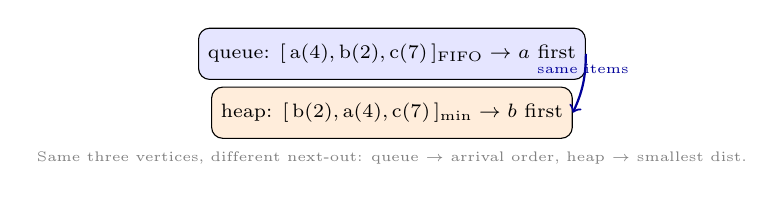
\begin{tikzpicture}[scale=0.68,every node/.style={font=\scriptsize}]
\node[draw,rounded corners,fill=blue!10,minimum width=3.2cm,minimum height=0.65cm] (q) at (0,0.5) {queue: [\,a(4),\,b(2),\,c(7)\,]$_{\rm FIFO}\to a$ first};
\node[draw,rounded corners,fill=orange!14,minimum width=3.2cm,minimum height=0.65cm] (h) at (0,-0.6) {heap: [\,b(2),\,a(4),\,c(7)\,]$_{\rm min}\to b$ first};
\draw[->,thick,blue!60!black] (q.east) to[bend left=12] node[font=\tiny,above] {same items} (h.east);
\node[font=\tiny,gray,align=center] at (0,-1.45) {Same three vertices, different next-out: queue $\to$ arrival order, heap $\to$ smallest dist.};
\end{tikzpicture}\caption{Queue vs heap: Dijkstra needs a priority line, not a fair line.}\label{fig:queue-vs-heap}\end{figure}
Heap implementation: binary heap gives $O((n+m)\log n)$; Fibonacci heap improves to $O(m+n\log n)$. Early exit when a target $t$ is extracted --- its distance is already final. Relaxation is the only place dist decreases, mirroring the BFS layering but weighted.

\begin{figure}[h]\centering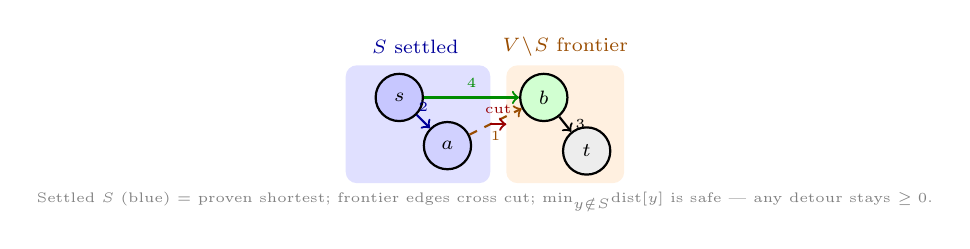
\begin{tikzpicture}[scale=0.68,every node/.style={font=\scriptsize}]
\fill[blue!12,rounded corners=4pt] (-2.6,-1.1) rectangle (0.1,1.1); \fill[orange!12,rounded corners=4pt] (0.4,-1.1) rectangle (2.6,1.1);
\node[circle,draw,thick,fill=blue!22,minimum size=6mm] (s) at (-1.6,0.5) {$s$}; \node[circle,draw,thick,fill=blue!18,minimum size=6mm] (a) at (-0.7,-0.4) {$a$}; \node[circle,draw,thick,fill=green!18,minimum size=6mm] (b) at (1.1,0.5) {$b$}; \node[circle,draw,thick,fill=gray!14,minimum size=6mm] (t) at (1.9,-0.5) {$t$};
\draw[thick,->,blue!60!black] (s)--(a) node[midway,above,font=\tiny] {2}; \draw[thick,->,green!55!black] (s)--(b) node[midway,above,font=\tiny] {4}; \draw[thick,->,orange!60!black,dashed] (a)--(b) node[midway,below,font=\tiny] {1}; \draw[thick,->] (b)--(t) node[midway,right,font=\tiny] {3};
\node[font=\scriptsize,blue!60!black] at (-1.3,1.45) {$S$ settled}; \node[font=\scriptsize,orange!60!black] at (1.5,1.45) {$V\!\setminus\! S$ frontier}; \draw[thick,red!60!black,->] (0.1,0) -- (0.4,0) node[midway,above,font=\tiny] {cut};
\node[font=\tiny,gray,align=center] at (0,-1.45) {Settled $S$ (blue) = proven shortest; frontier edges cross cut; $\min_{y\notin S}$dist$[y]$ is safe --- any detour stays $\ge0$.};
\end{tikzpicture}\caption{Dijkstra frontier: $S$ is the safe zone; the closest frontier vertex cannot be improved via a non-negative detour.}\label{fig:dijkstra-frontier}\end{figure}
\textit{Correctness --- invariant:} At the start of each iteration with $S$ already settled,
\begin{center}
(I)\quad $\forall\,x\in S:\ \text{dist}[x]=\delta(s,x)$ \quad and \quad $\forall\,y\notin S:\ \text{dist}[y]=\min_{P:\,s\to y\text{ with inner vertices in }S} w(P)$.
\end{center}
\emph{Initialisation:} $S=\emptyset$, (I) holds vacuously (dist$[s]=0$). \emph{Maintenance:} Let $u\notin S$ have minimum dist among $V\setminus S$. Any $s\to u$ path must leave $S$ at some edge $(x,y)$ with $x\in S$, $y\notin S$; its weight is $\ge \text{dist}[y]\ge\text{dist}[u]$ because all weights are non-negative, so no unseen path beats dist$[u]$. Extracting $u$ preserves (I) after relaxing its edges. \emph{Termination:} $S=V$ gives dist$[v]=\delta(s,v)$ for all $v$. If $w$ has a negative edge the inequality fails and Dijkstra may err --- a standard counterexample is $s\xrightarrow{2}b\xrightarrow{-2}a$ where $a$ is settled too early.

\subsection{Bellman--Ford: Relaxation and Negative Cycles}
No non-negativity needed. Relax every edge $n-1$ times, in any order:

\begin{quote}\ttfamily\small
\textbf{for} $i\gets1$ \textbf{to} $n-1$ \textbf{do} \textbf{for} each $(u,v)\in E$ \textbf{do} \textsc{Relax}$(u,v)$
\end{quote}

After $k$ rounds, dist$[v]$ equals the shortest weight among $s\to v$ paths using $\le k$ edges (induction on $k$: the $k$-edge optimum extends a $(k-1)$-edge optimum by one relaxation). Since any shortest simple path uses at most $n-1$ edges, after $n-1$ rounds dist$=\delta$ iff no negative cycle is reachable. One extra round detects one: if any relaxation succeeds, a negative cycle exists and $\delta=-\infty$ on its reachable vertices; tracing parent pointers retrieves it.

\begin{example}[Bellman--Ford detects a negative cycle]
Vertices $\{s,a,b\}$ with $s\xrightarrow{1}a,\ a\xrightarrow{1}b,\ b\xrightarrow{-3}a$. After $n-1=2$ rounds dist$[a]=1$, dist$[b]=2$. Round~3 relaxes $b\to a$: dist$[a]>2+(-3)=-1$, so dist$[a]$ drops --- negative cycle $a\to b\to a$ of weight $-2$ detected.
\end{example}

Time $O(nm)$, space $O(n)$ --- slower than Dijkstra but fully general.

\subsection{Floyd--Warshall: DP over Intermediate Vertices}
For all-pairs shortest paths, let $d^{(k)}[i,j]$ be the shortest $i\to j$ weight whose \emph{inner} vertices lie in $\{1,\dots,k\}$ (endpoints unrestricted). Then
\[
d^{(0)}[i,j]=\begin{cases}0&i=j\\w(i,j)&(i,j)\in E\\\infty&\text{else}\end{cases},\qquad
d^{(k)}[i,j]=\min\bigl(d^{(k-1)}[i,j],\ d^{(k-1)}[i,k]+d^{(k-1)}[k,j]\bigr).
\]
Iterating $k=1\ldots n$ in place (a single $n\times n$ matrix suffices since $d^{(k)}[i,k]=d^{(k-1)}[i,k]$ and $d^{(k)}[k,j]=d^{(k-1)}[k,j]$) yields $\delta(i,j)=d^{(n)}[i,j]$. Time $\Theta(n^3)$, space $\Theta(n^2)$. Negative-cycle check: $\exists\,i:\ d^{(n)}[i,i]<0$. Despite cubic cost, Floyd is concise, cache-friendly, and reconstructs paths via a successor matrix $\text{nxt}[i,j]$ updated alongside $d$.
\begin{remark}[Choosing among shortest-path algorithms]
Non-negative weights and single source: Dijkstra. Negative weights or cycle detection needed: Bellman--Ford. Dense all-pairs or transitive closure: Floyd--Warshall. On sparse graphs, running Dijkstra from each source with a heap can beat Floyd at $O(n(m\log n))$.
\end{remark}

% ============================================================
\section{String Matching}
\label{sec:string}
Text $T[1\ldots n]$, pattern $P[1\ldots m]$, alphabet $\Sigma$ ($n\ge m$). Report all shifts $s$ with $T[s+1\ldots s+m]=P$. We compare three strategies that trade comparison cost for preprocessing.

\subsection{Na\"ive \texorpdfstring{$\Theta((n-m+1)m)$}{Theta((n-m+1)m)} Scan}
Slide $P$ over each alignment $s=0\ldots n-m$ and compare $P[1\ldots m]$ against $T[s+1\ldots s+m]$ character by character, breaking on first mismatch. Worst case $\Theta((n-m+1)m)$ --- e.g., $T=a^n$, $P=a^{m-1}b$ forces $m$ comparisons at each of $n-m+1$ positions. No preprocessing, $O(1)$ extra space. The next two algorithms avoid re-scanning characters already matched.

\subsection{KMP: Prefix Function and Automaton}
\paragraph{Border = overlap.} For $P=\mathtt{abab}$, prefix $\mathtt{ab}$ = suffix $\mathtt{ab}$ --- it \emph{borders} the string. On mismatch you slide the pattern so the longest border that still matches the text suffix stays aligned; you do not restart at $0$.
\begin{figure}[h]\centering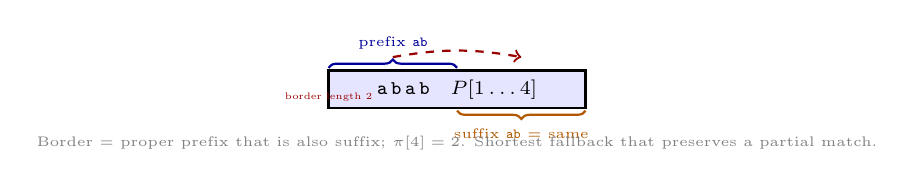
\begin{tikzpicture}[scale=0.68,every node/.style={font=\scriptsize}]
\draw[thick,fill=blue!10] (0,0) rectangle (4.8,0.7); \node at (2.4,0.35) {$\mathtt{a\,b\,a\,b}$ \; $P[1\ldots4]$};
\draw[thick,blue!60!black,decorate,decoration={brace,amplitude=3pt}] (0,0.75) -- (2.4,0.75) node[midway,above=3pt,font=\tiny] {prefix $\mathtt{ab}$};
\draw[thick,orange!70!black,decorate,decoration={brace,amplitude=3pt,mirror}] (2.4,-0.05) -- (4.8,-0.05) node[midway,below=3pt,font=\tiny] {suffix $\mathtt{ab}$ = same};
\draw[->,thick,red!60!black,dashed] (1.2,0.95) to[bend left=10] (3.6,0.95) node[midway,above,font=\tiny] {border length 2};
\node[font=\tiny,gray,align=center] at (2.4,-0.65) {Border = proper prefix that is also suffix; $\pi[4]=2$. Shortest fallback that preserves a partial match.};
\end{tikzpicture}\caption{Border picture for $\mathtt{abab}$ --- the overlap that lets KMP fall back instead of restarting.}\label{fig:kmp-border}\end{figure}
Let $\pi[q]=\max\{k<q: P[1\ldots k]\text{ is suffix of }P[1\ldots q]\}$ for $1\le q\le m$ ($\pi[1]=0$); equivalently $\pi[q]$ is the longest proper border of the prefix $P[1\ldots q]$. Computed in $O(m)$ by amortised fallback:

\begin{quote}\ttfamily\scriptsize
$\pi[1]\gets0;\ k\gets0$; \textbf{for} $q\gets2$ \textbf{to} $m$: \textbf{while} $k>0\land P[q]\neq P[k+1]$ do $k\gets\pi[k]$; \textbf{if} $P[q]=P[k+1]$ then $k\gets k+1$; $\pi[q]\gets k$
\end{quote}

Matching scans $T$ once, maintaining $q$ = length of longest prefix of $P$ that is a suffix of $T[1\ldots i]$; on mismatch fall back $q\gets\pi[q]$. Total $O(n+m)$ time, $O(m)$ extra space; each character of $T$ is examined at most twice.

The automaton view: state $q$ means ``first $q$ characters of $P$ just matched.'' Transition $\delta(q,c)$ is the longest prefix of $P$ that is a suffix of $P[1\ldots q]c$; missing edges follow $\pi$-links (failure function).

\begin{figure}[h]\centering
\begin{tikzpicture}[->,>=Stealth,shorten >=1pt,auto,node distance=1.9cm,semithick]
\tikzstyle{state}=[circle,draw,thick,minimum size=7mm,font=\small] \tikzstyle{spine}=[->,>=Stealth,thick,blue!70!black] \tikzstyle{fail}=[->,>=Stealth,thick,dashed,red!60!black]
\node[state,initial,initial text={},fill=blue!12] (0) {$0$}; \node[state,fill=blue!8] (1) [right of=0] {$1$}; \node[state,fill=blue!8] (2) [right of=1] {$2$}; \node[state,fill=blue!8] (3) [right of=2] {$3$}; \node[state,accepting,fill=green!15] (4) [right of=3] {$4$};
\path[spine] (0) edge[bend left=10] node[font=\scriptsize,above] {a} (1) (1) edge[bend left=10] node[font=\scriptsize,above] {b} (2) (2) edge[bend left=10] node[font=\scriptsize,above] {a} (3) (3) edge[bend left=10] node[font=\scriptsize,above] {b} (4);
\path[spine] (1) edge[loop above] node[font=\scriptsize] {a} (1);
\path[fail] (2) edge[bend left=30] node[font=\scriptsize,below] {a} (1) (3) edge[bend left=30] node[font=\scriptsize,below] {b} (2) (4) edge[bend left=38] node[font=\scriptsize,below] {b} (2) (4) edge[bend left=20] node[font=\scriptsize,above] {a} (3);
\end{tikzpicture}
\caption{KMP automaton for $P=\mathtt{abab}$ ($m=4$). Solid spine spells $P$; failure links (merged into $\delta$) redirect on mismatch via $\pi$: $\pi=[0,0,1,2]$. Scanning $T$ never moves backwards, giving $O(n+m)$ time.}
\label{fig:kmp-automaton}
\end{figure}

\subsection{Rabin--Karp: Rolling Hash}
\paragraph{Clock arithmetic.} Working $\bmod\,q$ is like a clock with $q$ hours: after $q-1$ you wrap to $0$. Adding or multiplying then taking $\bmod\,q$ discards full laps but preserves remainders; collisions are two different strings landing on the same hour mark. A large prime $q$ makes accidental collisions rare.
Treat strings as base-$b$ numbers modulo a prime $q$. Let $h(s)=T[s+1\ldots s+m]\bmod q$ and $p=P\bmod q$. With precomputed $b^{m-1}\bmod q$,
\[
h(s+1)=\bigl(b\cdot(h(s)-T[s+1]\cdot b^{m-1})+T[s+m+1]\bigr)\bmod q,
\]
so each shift is $O(1)$ after $O(m)$ preprocessing. If $h(s)\neq p$ there is no match; if equal, verify by direct comparison (handles spurious hits from collisions). Expected $O(n+m)$ with good $q$ and $O(nm)$ worst case when every window collides.

\begin{example}[Rolling hash by hand]
Let $b=10$, $q=13$ (small for illustration), $T=\mathtt{31415}$, $m=2$. Then $h(0)=\mathtt{31}\bmod13=5$, $h(1)=(10\cdot(5-3\cdot10)+\mathtt{4})\bmod13=1$ which equals $\mathtt{14}\bmod13=1$; $p=\mathtt{15}\bmod13=2$, so neither window matches $P=\mathtt{15}$. With real $b=256$, $q\approx10^9+7$ and Horner evaluation, the same recurrence applies to strings over bytes.
\end{example}

Double hashing (or $q\gg n$) makes collisions negligible; one text scan then serves 2-D and multi-pattern search such as plagiarism detection over a corpus.

% ============================================================
\section{Maximum Flow: Ford--Fulkerson and Min Cut}
\label{sec:maxflow}
\paragraph{Pipes and water.} Picture each directed edge as a pipe stamped with its capacity: how much water per second it can carry from a source $s$ to a sink $t$. A \emph{flow} assigns a rate to every pipe so that no pipe bursts (flow $\le$ capacity) and every junction except $s$ and $t$ passes on exactly what it receives (inflow $=$ outflow). The goal is to push as much water as possible from $s$ to $t$.
\begin{definition}[Flow network and flow] A flow network is a directed graph with capacities $c(u,v)\ge 0$ ($0$ if no edge), source $s$ and sink $t$. A flow $f$ obeys $0\le f(u,v)\le c(u,v)$ and conservation $\sum_u f(u,v)=\sum_w f(v,w)$ for all $v\notin\{s,t\}$; its value is $|f|=\sum_v f(s,v)$.
\end{definition}
\paragraph{Residual graph: the room that is left.} Given $f$, the \emph{residual capacity} $c_f(u,v)=c(u,v)-f(u,v)+f(v,u)$ says how much more can still go $u\to v$: spare room forward, plus already-sent flow that could be cancelled backwards. Edges with $c_f>0$ form the residual graph $G_f$; any $s\to t$ path $P$ in $G_f$ (an \emph{augmenting path}) carries bottleneck $\Delta=\min_{(u,v)\in P}c_f(u,v)$ extra units.
\begin{quote}\ttfamily\scriptsize
\textsc{Ford--Fulkerson}: $f\gets0$; \textbf{while} an $s\to t$ path $P$ exists in $G_f$ \textbf{do} augment $f$ along $P$ by bottleneck $\Delta=\min c_f$.
\end{quote}
\begin{figure}[h]\centering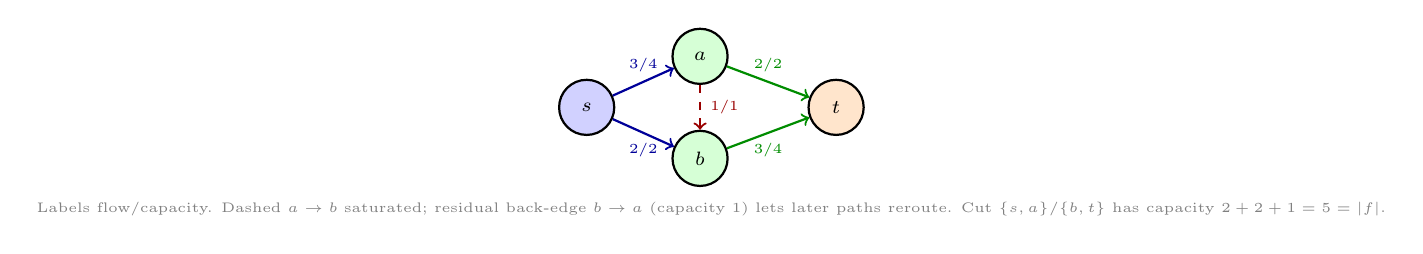
\begin{tikzpicture}[scale=0.72,every node/.style={font=\scriptsize}]
\node[circle,draw,thick,fill=blue!18,minimum size=7mm] (s) at (0,0) {$s$}; \node[circle,draw,thick,fill=green!16,minimum size=7mm] (a) at (2,0.9) {$a$}; \node[circle,draw,thick,fill=green!16,minimum size=7mm] (b) at (2,-0.9) {$b$}; \node[circle,draw,thick,fill=orange!20,minimum size=7mm] (t) at (4.4,0) {$t$};
\draw[thick,->,blue!60!black] (s)--(a) node[midway,above,font=\tiny] {3/4}; \draw[thick,->,blue!60!black] (s)--(b) node[midway,below,font=\tiny] {2/2}; \draw[thick,->,green!55!black] (a)--(t) node[midway,above,font=\tiny] {2/2}; \draw[thick,->,green!55!black] (b)--(t) node[midway,below,font=\tiny] {3/4}; \draw[thick,->,red!60!black,dashed] (a)--(b) node[midway,right,font=\tiny] {1/1};
\node[font=\tiny,gray,align=center] at (2.2,-1.8) {Labels flow/capacity. Dashed $a\to b$ saturated; residual back-edge $b\to a$ (capacity~1) lets later paths reroute. Cut $\{s,a\}{/}\{b,t\}$ has capacity $2+2+1=5=|f|$.};
\end{tikzpicture}\caption{A flow of value~5 with residual back-edge; the dashed cut certifies optimality via max-flow min-cut.}\label{fig:maxflow}\end{figure}
\begin{example}[Three augmentations] Capacities as in Fig.~\ref{fig:maxflow}. Augment $s\to a\to t$ by $2$ (bottleneck $a\to t$), then $s\to b\to t$ by $2$, then $s\to a\to b\to t$ by $1$ through $a\to b$. Now the residual reach of $s$ is $\{s,a\}$ only, so no augmenting path remains and $|f|=2+2+1=5$ is maximum.
\end{example}
\begin{theorem}[Max-flow min-cut] For every network, the maximum flow value equals the minimum capacity $\sum_{u\in S,v\notin S}c(u,v)$ over all $s$--$t$ cuts $(S,V\setminus S)$. Ford--Fulkerson terminates with a maximum flow for integer capacities in $O(m\cdot|f^*|)$ time; always augmenting along a shortest path (Edmonds--Karp BFS) costs $O(nm^2)$ and works for irrational capacities too.
\end{theorem}

% ============================================================
\section{Chapter Notes}
BFS (Moore, 1959) and DFS (Tarjan, 1972) in modern form underpin all graph algorithms. Dijkstra (1959) with binary heaps is the practical default; Bellman--Ford (1958) and Floyd--Warshall (1962) handle negative weights. KMP (Knuth--Morris--Pratt, 1977) and Rabin--Karp (1987) remain textbook representatives of automaton vs.\ hashing; maximum flows and minimum cuts are CLRS Ch.~26. CLRS Chs.~20--24, 32 covers all topics in depth.

% ============================================================
\section{Exercises}
\label{sec:ch07-exercises}
\begin{enumerate}[label=E7.\arabic*, leftmargin=*, itemsep=0.8em]
    \item \textbf{BFS layering vs.\ DFS depth.} Run BFS and DFS (alphabetical adjacency) from $s$ on the graph of Fig.~\ref{fig:bfs-tree} with extra edge $e\to a$. List discovery order, dist$[\cdot]$ from BFS, and DFS finish times $f[\cdot]$. Give a graph where DFS from $s$ never discovers a vertex that BFS does. Can that happen if the graph is undirected and connected? Justify.

    \item \textbf{Dijkstra proof in action.} (a) Execute Dijkstra with a binary heap from $s$ on: $s\!\xrightarrow{4}\!a,\ s\!\xrightarrow{2}\!b,\ b\!\xrightarrow{1}\!a,\ a\!\xrightarrow{3}\!t,\ b\!\xrightarrow{5}\!t$. Show heap contents per extraction and invariant~(I). (b) Add edge $b\xrightarrow{-3}a$ and show extraction order violates (I) and yields a wrong distance. (c) Would Bellman--Ford recover the correct distances and how many rounds suffice?

    \item \textbf{KMP prefix function.} (a) Compute $\pi$ for $P=\mathtt{aabaaab}$ step by step. (b) Draw the KMP automaton states $0\ldots7$ and label failure ($\pi$) links. (c) Trace KMP on $T=\mathtt{aabaabaaab}$ and count character comparisons versus na\"ive scan. Prove $O(n+m)$ is tight by giving a family attaining $\Theta(n+m)$ comparisons.

    \item \textbf{Rolling hash design.} Let $b=256$, $q=101$. (a) Compute the Rabin--Karp hash of $P=\mathtt{abc}$ and the rolling update to the next window in $T=\mathtt{abcd}$. (b) Exhibit $P\neq Q$ over $\{a,b\}$ colliding modulo $101$, and explain why a second modulus $q_2$ reduces collision probability to $\approx 1/(q\,q_2)$. (c) Argue expected time is $O(n+m)$ when $q\ge m^2$ and verification is $O(m)$, assuming uniform hashing.

    \item \textbf{Max flow and min cut.} (a) Starting from zero flow on Fig.~\ref{fig:maxflow}, list the residual graph $G_f$ and bottleneck $\Delta$ for each of the three augmentations in the worked example. (b) Verify cut $\{s,a\}{/}\{b,t\}$ has capacity~5 and prove no flow can exceed any $s$--$t$ cut capacity. (c) Give integer capacities where a poor augmenting-path choice needs $\ge 10$ augmentations while Edmonds--Karp (BFS paths) finishes in $2$; state both runtimes.
\end{enumerate}
% End of Chapter 7
